% file: vlsi-binary-tree.tex

\documentclass{standalone}
\usepackage{tikz}
\usepackage{tikz-qtree}
\usetikzlibrary{shapes}

\begin{document}
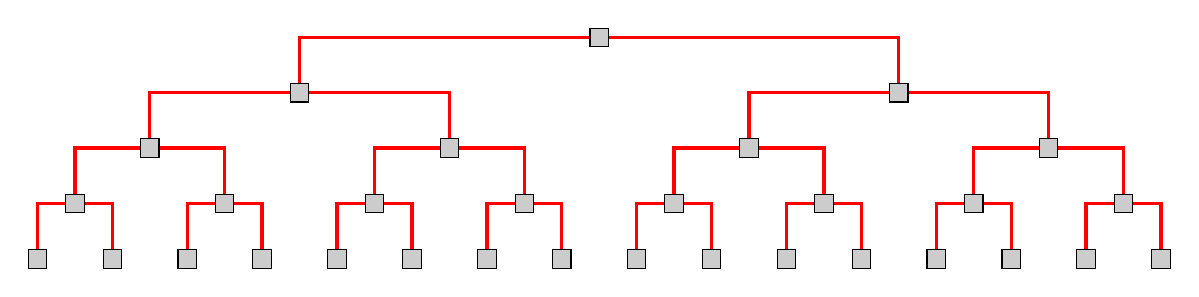
\begin{tikzpicture}[level distance = 20pt, sibling distance = 20pt]
\tikzset{edge from parent/.style= {draw, red, very thick, 
  	edge from parent path = {(\tikzparentnode) -| (\tikzchildnode)}},
    every tree node/.style = {draw, rectangle, fill = gray!40}}
    \Tree [.{} 
	    [.{}
	      [.{} 
		[.{} 
		  [.{} ]
		  [.{} ]
		]
		[.{} 
		  [.{} ]
		  [.{} ]
		]
	      ] 
	      [.{} 
		[.{} 
		  [.{} ]
		  [.{} ]
		]
		[.{} 
		  [.{} ]
		  [.{} ]
		]
	      ] 
	    ]
	    [.{} 
	      [.{} 
		[.{} 
		  [.{} ]
		  [.{} ]
		]
		[.{} 
		  [.{} ]
		  [.{} ]
		]
	      ]
	      [.{} 
		[.{} 
		  [.{} ]
		  [.{} ]
		]
		[.{} 
		  [.{} ] 
		  [.{} ] 
		]
	      ] 
	    ]
         ]
\end{tikzpicture}
\end{document}